%
% include the class file for USI-INF Technical Reports
%
\documentclass{usiinftr}
\usepackage{float}
\usepackage{amsmath}
\usepackage{slashbox}
\usepackage{subfigure}
\usepackage{listings}
\usepackage{algorithm}
\usepackage{algorithmicx}
\usepackage[noend]{algpseudocode}

%%%%%%%%%%%%%%%%%%%%%%%%%%%%%%%%%%%%%%%%%%%%%%%%%%%%%%%%%%%%%%%%%%%%
\newcommand{\der}{\operatorname{d\!}{}}
\begin{document}

\title{\bf Bayesian Added Regression Tree (BART) \\ {\normalfont An overview of applications of Bayesian methods in regression }}
\author{Glejdis Shk\"embi}{\dagger}
\author{Franciskus Xaverius Erick}{\dagger}

\affiliation{\dagger}{Faculty of Engineering, Friedrich-Alexander Universit\"at Erlangen-N\"urnberg, Germany}

%
% by default, the current month and year are used as the publication date
% of your Technical Report; if you want to change this, then you can do it here, e.g.
%
%\date{February~\the\year}
%\date{August 2011}

\maketitle

\begin{abstract}

\end{abstract}

\section{Motivation}
.
\section{Mathematical Background}
In its core the FFT is an algorithm that allows us to solve a mathematical problem with less computational effort than needed at first glance.
It calculates the discrete Fourier transform (DFT), which can be described as a matrix vector multiplication in only $\mathcal{O}(n\log(n))$ operations\cite{cochran1967fast}. 

In this section we will provide the most important mathematical basics of the FFT. We will cover the notion of Hilbert spaces, which gives a framework for function spaces and the understanding of functions as bases.
Furthermore, we will introduce the main aspects of the Fourier series and transform in their analytical and discrete form.

\subsection{Classification and Regression Trees - CART}
The Classification and Regression Tree analysis, first introduced by Breiman et al. in 1984, is a well known decision tree method used in constructing predictor variables from the data. It builds a binary decision tree based on some splitting rule on the predictors [1]. Regression trees are used for variables with continuous or ordered discrete values, while classification trees are intended for variables with a finite number of unordered values. Moreover, for regression trees, the prediction error is commonly assessed as the squared difference between the observed and predicted values, while for classification trees the prediction error is evaluated in terms of misclassification cost [2].

In a classification task, we have a training set with n observations, a class variable Y such that Y $\in {1, 2, \cdots, k}$ and the predictor variables $X_1, \cdots ,X_p$ with fixed dimensionality p and we try to find a model that better predicts the class Y given new values of X [1]. The CART technique for classification problems produces rectangular sets $A_j$ by recursively partitioning the data set a single X variable at a time into disjoint sets $A_1,\cdots, A_j$ and fitting a single prediction model within each partition [2]. The partitioning is repeated until a node is reached for which no split enhances homogeneity, at which point splitting is stopped and this node becomes a terminal node [1]. This partitioning can be visually represented with a decision tree. In figure 1.0 we see a classification tree model with three classes labeled 1, 2 and 3, where the partitions are on the left and the decision tree is on the right. The root node of the tree represents the entire data set, and at each node, if the condition is satisfied, a case is assigned to the left child node. Moreover, the predicted class is beneath each leaf node [2]. In contrast, in a regression task, the Y variable takes ordered values and we are trying to fit to each node a regression model to give predicted values of Y [2].

The algorithm starts at the root node of the tree and grows itself as follows [3]: 
\begin{itemize}
\item Step 1: Explore every possible split on each predictor variable. Binary questions are typically used to produce binary splits.
\item Step 2: Select and apply the best split (ie. selects the best feature which helps us better predicting the target class).
\item Step 3: Recursively proceed in this way until a stopping criterion is reached. 
\end{itemize}

The stopping criterion is reached when [4]:
\begin{itemize}
\item The node's examples all belong to the same class.
\item There are no features remaining to distinguish between samples.
\item The tree has grown to the predetermined size limit. 
\item The first problem for a decision tree is determining which feature to split on.
\end{itemize}

Purity refers to the degree to which a subset of examples contains just a single class, and any subset made of only a single class is pure [4]. There are several purity metrics that may be used to choose the optimal decision tree splitting candidate. C5.0 and CART are two algorithms for classification that follow this approach. They are both very similar, however, C5.0 uses entropy for its impurity measure, while CART uses the Gini index [2]. Entropy is a measure of randomness or disorder within a set of class values. Mathematically, the entropy is formulated as follows: 
,
where S represents the segment of data, c the number of different classes and p the probability of the values being part of class i [4]. When entropy is equal to 0, this indicates that the set is completely homogeneous. The higher the entropy, the more diverse the set is, which means that less information is provided about other data points that may belong in the set. The goal of C5.0 is to find splits that reduce entropy,  hence enhancing homogeneity within the groups [4]. Now, using entropy, the Information Gain of a feature F can be calculated as shown below[4]:

The higher the information gain is, the more homogeneous the set created after the split on this feature is. On the other hand, Gini index calculates the "impurity" of a feature with respect to the classes [5]. More specifically, it indicates the probability of a specific feature to be classified incorrectly when we do random selection. It is given by the following formula [5]:

Breiman et al. (1984) points out that the stopping rules in Step 3 do not work very well in practical applications, as the tree tends to become too large and has too few data points in each terminal node, making its decisions overly specific and increasing the risk of model overfitting. Therefore, to address this issue, there is the need to prune the tree. Pruning a decision tree is the process of reducing its size in order to generalize better to unseen data [4]. There are two types of decision tree pruning: pre-pruning or post-pruning. In pre-pruning, also known as early stopping, we let the tree grow until it reaches a predefined number of decisions or until there is only a small number of examples in the node, and then we stop it [4]. In this way we avoid doing extra work, however, it is difficult to know whether this way we leave out subtle but important patterns. On the other hand, in post-pruning, we intentionally allow a very large tree to grow and then we use pruning criteria to reduce its size to a more appropriate level [4]. This type of pruning ensures us that all of the important information is discovered. 
	
Some of the main advantages of the decision trees include [4]:
\begin{enumerate}
\item Are easy to be interpreted even by non-statisticians;
\item Work well with missing variables;
\item Are invariant under transformations in the predictor space;
\item There are extensions: Bayesian version of CART.
\end{enumerate}

Moreover, some of the drawbacks are:
\begin{enumerate}
\item A lot of data is needed as the tree-space is big;
\item Might not result in the "best" model;
\item There is selection bias for the splits;
\item May lead to overfitting.
\end{enumerate}

\subsection{Markov Chain Monte Carlo - MCMC}
In Bayesian statistics, one would normally propose a prior distribution of the samples and these priors are updated according to the likelihood of observations from the samples. In this way, the posterior distribution, which describes the the distribution of the samples given the obtained likelihood, can be determined. The main formula of this update process is given as follows.

\begin{equation} \label{Bayes}
p(\theta \mid y) = \frac{p(\theta)p(y \mid \theta}{p(y)} = \frac{p(\theta)p(y \mid \theta}{\int p(\theta)p(y \mid \theta d\theta}
\end{equation}

The integral in the denominator which represents the marginal likelihood of y can be treated as a normalizing constant of the whole expression. For very simple distributions, this normalizing constant can be determined analytically. However, in real life situations, the likelihoods obtained can get highly complex in expression,which makes it impossible to evaluate this integral term. There are various methods that can be used instead to approximate the posterior distribution, without the need to evaluate such complicated integrals. One of the most common method is Markov Chain Monte Carlo, or MCMC.

Markov Chain Monte Carlo, first introduced by physicists at Los Alamos in the 1940's, is a computer-based sampling approach, which, by randomly sampling values out of the distribution, allows one to describe a distribution without knowing in advance all of its mathematical properties [20]. As written in the name, MCMC combines two properties: Monte Carlo and Markov Chain. 

Monte Carlo estimates the properties of a distribution by exploring random samples from the distribution, while Markov Chain generates random samples sequentially where each random sample is used as a building block to generate the next random sample [20]. In other words, rather than computing the mean of a normal distribution from its equations, in Monte Carlo approach we draw a large number of random samples from this normal distribution and then compute the sample mean, which is much easier than computing the mean directly from the normal distribution's equations.

Markov Chain is a sequence $X_1,X_2, X_3, \cdots$ of random variables if the conditional distribution of $X{n+1}$ given $X_1,X_2, X_3, \cdots, X_n$ depends only on $X_n$ [21].That is to say that the future is independent of the past given the present [21]. This is known under the name of Markov Property. In MCMC, the state of the Markov chain $\theta^{t}$ is a drawn sample that corresponds to a certain distribution at iteration step $t$. Due to the Markovian property, the states at current iteration only depends on the states of the previous iteration step. The goal of MCMC is to simulate the posterior distribution $p(\theta \mid y)$, which can be treated as the target distribution, by iteratively constructing Markov Chain which stationary distribution converges to the target posterior distribution. 


\subsection{Metropolis-Hastings algorithm}
Computationally, the generation of Markov chains in MCMC can be realized through Metropolis-Hastings algorithm. Metropolis-Hastings algorithm employs proposal distribution $q(\theta^{t},\theta^{t-1})$, from which each state $\theta^{t}$ at iteration step $t$ is proposed, eventually leading to the desired Markov chain. The proposed state depends on the state from the previous iteration $\theta^{t+1}$. With Metropolis-Hastings algorithm, one would be able to approximate any probability density function $\pi(x)$ using only a proposal distribution function $q(x)$ and a function $f(x)$ which is proportional to the real probability density function $\pi(x)$.  This is especially useful in the context of approximating posterior distribution function as of \ref{Bayes}. Since the posterior distribution is proportional to the numerator of the right hand side of the equation, one would only need to evaluate the numerator and propose a proposal distribution to approximate the posterior distribution by Metropolis-Hastings algorithm, without the need to analytically compute the complex integral in the denominiator.

In general, the symmetric Metropolis-Hastings ( $q(x_t,x_{t-1}) = q(x_{t-1},x_t)$ ) algorithm with proposal distribution function $q(x)$ and function $f(x)$ can be described in the following pseudocode.

\begin{algorithm}
  \caption{General Metropolis-Hastings algorithm} \label{algMH}
  \begin{algorithmic}[1]
    \Statex
    \Function{MH}{$x_0, n$}
    \State {$x_1 = x_0$}
    \For { $i \gets 2 \textrm{ to }  n $ }
    	\State { $ y \gets q(x_i,x_{i-1})$ }
    	\State { $ \alpha \gets \textrm{min}(1, f(y)/f(x_{i-1}))$ }
    	\State { $ u \gets \textrm{runif}(1) $}
    	\If { $ \alpha \geq u $ }
    		\State{ $ x_i = y$}
        \Else
            \State{ $ x_i = x_{i-1}$}
        \EndIf
    \EndFor
    \State \Return{$x$}
    \EndFunction
  \end{algorithmic}
\end{algorithm}

In the pseudocode, the first state is initialized with a given initial state. The candidate next state is then proposed from the proposal distribution given the previous state. The acceptance ratio $\alpha$ evaluate the probability of moving from the current state to the candidate state. If this acceptance ratio value is lower than a randomly generated number from a uniform distribution ranging from 0 to 1, then the candidate state is taken as the next state. Otherwise, the next state would simply just be the current state ( no move from the current state ). This is iterated until a maximum number of iteration $n$ is reached. In the case when the proposal distribution is not symmetric, the acceptance ratio would be $ \alpha \gets \textrm{min}\left(1, \frac{f(y)q(y,x_{i-1})}{f(x_{i-1})q(x_{i-1},y}\right)$ instead. 

Since the proposal distribution depends on the previous state, this very algorithm is also a case of random walk Metropolis Hasting. The Metropolis-Hasting algorithm is relatively easy to implement and does not suffer from curse of dimensionality, which is a well known issue for importance and rejection sampling. Therefore, the Metropolis-Hastings is currently very widely used for Bayesian inference. 

A convergence to the target distribution is also guaranteed. However, care needs to be taken of with regards to the proposal distribution used. If the variance of the proposal distribution is too low, the states proposed would be too close and similar to each other, resulting to a higher degree of autocorrelation and subsequently a slow convergence. If the variance of the proposal is too high, there would also be a higher amount of rejected candidates, which in turn result to slow convergence. To ensure that the final distribution is indeed approximate to the target distribution, a burn-in period is also taken into consideration. This means that the proposed states from the first $n$ ( typically 1000 iterations ) are ignored as the initial distributions may not reflect the true converged target distribution.


\subsection{Gibbs Sampler} 
Gibbs sampling can be considered to be a special case of Metropolis-Hastings algorithm, whereby the acceptance rate is always taken as 1. It is specially used when sampling multivariate distributions, whereby a "correct" proposal distribution function that ensures reasonable convergence speed may not be easily determined. For Gibbs sampling, the update of each dimension of the state $\theta^{t}_d$ is given as the conditional distributions of each dimension for the dimensions $d = 1,2,\cdots,D$. In general, Gibbs sampling algorithm is done in the following pseudo-code:

\begin{algorithm}[h]
  \caption{General Gibbs sampler algorithm} \label{algGibbs}
  \begin{algorithmic}[1]
    \Require{The initial state of $\theta$ has already been initialized,$ \theta^{1} \neq \textrm{NULL}$}
    \Statex
    \Function{Gibbs}{$\theta, n$}
    \For { $i \gets 2 \textrm{ to }  n $ }
    	\State { $ \theta_1^{i} \gets \pi( \theta^{i}_1 \mid \theta^{i-1}_{2},\theta^{i-1}_{3}, \theta^{i-1}_{4}, \cdots, \theta^{i-1}_{D} )$ }
    	\State { $ \theta_2^{i} \gets \pi( \theta^{i}_2 \mid \theta^{i}_{1},\theta^{i-1}_{3},\theta^{i-1}_{4}, \cdots, \theta^{i-1}_{D} )$ }
    	\State { $ \theta_3^{i} \gets \pi( \theta^{i}_3 \mid \theta^{i}_{1},\theta^{i}_{2},\theta^{i-1}_{4}, \cdots, \theta^{i-1}_{D} )$ }
    	\State { $ \vdots $ }
    	\State { $ \theta_D^{i} \gets \pi( \theta^{i}_D \mid \theta^{i}_{1},\theta^{i}_{2},\theta^{i}_{4}, \cdots, \theta^{i}_{D-1} )$ }
    \EndFor
    \State \Return{$\theta$}
    \EndFunction
  \end{algorithmic}
\end{algorithm}

Thus for Gibbs sampler, one would only required the conditional distributions in order to approximate the 
target distribution. As the acceptance rate is always 1, no additional proposal distribution matching is required. However, this method can only be done when the conditional distributions can be sampled from. This is always not the case as for some distributions, the conditional distribution expressions can even be hard to obtain. Furthermore, the acceptance rate of 1 also comes with the cost of the inability to adapt to the cases when the states are highly correlated ( high autocorrelation ). This would also lead to a slower convergence as the high correlation would makes it harder for the algorithm to cover the whole target distribution. As in the classic Metropolis-Hastings algorithm, burn-periods need to be taken into account to ensure convergence of the Markov Chain.

\subsection{Bayesian Added Regression Tree}
As previously mentioned, the classical CART is prone to overfitting. This leads to various research into a more Bayesian approach to the decision trees. By applying Bayesian framework, the data can overcome the assumptions about the depth of trees and the shrinkage needed. The Bayesian framework encodes what is typically an algorithmic approach in a likelihood framework to generate coherent uncertainty intervals, which is uncommon for machine learning methods. 

 Chipman et al. (2010) proposed a Bayesian "sum-of-trees" model, which is defined by a prior and a likelihood, where each tree is constrained by a regularization prior in order to be a weak learner.  Fitting is achieved by a specialized iterative backfitting MCMC algorithm. This "sum-of-trees" model results to be adaptive and very flexible, where each individual tree describes a different part of the underlying mean function [7]. The "sum-of-trees" model differ from other ensemble methods that fit a linear combination of trees, such as boosting [11], random forests [10], bagging [12]. In bagging and random forest models we do random sampling and stochastic search to create a collection of independent trees, and then combine their results by averaging. It is worth noticing that from various literatures, BART performs better compared to LASSO [8], gradient boosting [9], random forests [10] and neural networks with one hidden layer. 
 
\subsubsection{Sum of Trees Model}
Chipman et al. (2010) consider the problem in which a dependent variable Y needs to be predicted using the p dimensional input vector $\textbf{x} = (x_1,\cdots, x_p)$:

\begin{equation}
Y=f(x)+\epsilon, \quad \epsilon \sim N\left(0, \sigma^{2}\right),
\end{equation}

where function f(x) is unknown. Bayesian statistics aims to approximate the mean of Y given x by the sum of m trees. Each tree is represented by the $g_j$ function:

\begin{equation} \label{sum}
f(x)=E(Y \mid x) \approx h(x) \equiv \sum_{j=1}^{m} g_{j}(x)
\end{equation}

We further break down the components of the trees in the $g_j$ function. We define $T_j$ to be the j-th tree with the corresponding terminal nodes $M_j = \{ \mu{ij}, \cdots, \mu{bj} \}$. b defines the amount of terminal nodes of the corresponding tree. Thus, equation \ref{sum} can be rewritten as follows.

\begin{equation} \label{sum1}
f(x)= \sum_{j=1}^{m} g(x;T_j,M_j)
\end{equation}

\subsubsection{Regularization Priors}
Bayesian priors are the main features in BART which enforce regularization to the added regression trees, thus ensuring that the trees do not get too significantly big, adapt to the data well while at the same time reduce overfitting. The prior specifications, stated in Chipman et al. (2010), will be described in more detail here.

There are three priors used for regularization, namely:
\begin{enumerate}
\item $\pi(T_j)$ the prior of the tree structure itself,
\item $\pi(M_j \mid T_j)$ the prior of the leaf structures given the tree structure, 
\item $p(\sigma^2)$ the residual variance.
\end{enumerate}

Each of the prior are discussed in more details as follows.
\begin{enumerate}
\item $\pi(T_j)$ the prior of the tree structure itself. This prior itself has 3 separate components
			\begin{enumerate}
				\item The probability that the node depth $d = 1,2,\cdots,n$ is not terminal. The node depth is defined as the distance from the root node. This is expressed as 
			\begin{equation}\frac{\alpha}{(1+d)^{\beta}}, \quad \alpha \in (0,1), \beta \geq 0 . \end{equation}
			Where $\alpha$ and $\beta$ are hyperparameters to be tuned. This component enforces regularization on the depth of the trees itself so that they do not get too large. Chipman et al. (2010) recommends default values of $\alpha = 0.95$ and $\beta =2$.
				\item The probability that the i-th feature out of p features of data is taken to be the decisive splitting variable for a node. Chipman et al. (2010) uses uniform distribution over all the possible features p.
				\item The probability that for the selected i-th feature , that a certain value of cut off point is used. Chipman et al. (2010) uses uniform distribution over all the discrete possible splitting values of that certain feature.
			\end{enumerate} 
\item The prior $\pi(M_j \mid T_j)$ can be expressed as the product of all probabilities of the observed terminal nodes given the tree.
\begin{equation}\pi(M_j \mid T_j) = \prod_i p(\mu_{ij} \mid T_j). \end{equation}

Chipman et al. (2010) recommends a normal distribution for the prior $p( \mu_{ij} \mid T_j) \sim \mathcal{N}(0, \sigma^2_{ \mu })$, whereby $ \sigma_{ \mu } = \frac{0.5}{k \sqrt{m}}$  and k is a hyperparameter to be tuned. The default value of k is taken as k = 2. Thus, this term would ensure that the leaves output get closer to 0 ( the center of the normal distribution ) when the variance term $\sigma_{ \mu}$ gets smaller.
\item $p(\sigma^2)$, which is the residual variance. This prior is modelled with the conjugate prior inverse chi square distribution, which is none other than a special case of inverse Gamma distribution, as follows.
\begin{equation}p(\sigma^2) \sim \frac{\nu \lambda}{\chi_{\nu}^2}. \end{equation}

With $\lambda$ and $\nu$ as the hyperparameters. More frequently, another hyperparameter is $q$ is chosen in order to determine the hyperparameter $\lambda$ from looking at the prior distribution. While there are more detailed approaches to choosing the hyperparameters, for convenience, Chipman et al. (2010) additionally suggests to use the default values of $\nu = 3$ and $q = 0.90$ to avoid overfitting and yield good results.
\end{enumerate}

Taking these prior components into account, the resulting regularization prior distribution is none other 
than:

\begin{equation}
\begin{aligned}
p\left(\left(T_{1}, M_{1}\right), \ldots,\left(T_{m}, M_{m}\right), \sigma\right) &=\left[\prod_{j} p\left(T_{j}, M_{j}\right)\right] p(\sigma) \\
&=\left[\prod_{j} p\left(M_{j} \mid T_{j}\right) p\left(T_{j}\right)\right] p(\sigma)
&= \left[\prod_{j}  \prod_{i} p\left(\mu_{i j} \mid T_{j}\right) p\left(T_{j}\right)\right] p(\sigma)
\end{aligned}
\end{equation}

The likelihood is taken to be the likelihood of outputting certain values of Y given the tree models with its specifications. This likelihood is modelled with a normal distribution, with the mean being the best guess possible for the specific configurations of the added regression trees.

\begin{equation}
y_l \sim \mathcal{N}(\mu_l, \sigma^2)
\end{equation}

\subsubsection{Posterior distributions}
With the priors and likelihood specified in the previous sections, the posterior distribution is now left to be approximated. Direct analytical evaluation of the posterior distribution is not possible as it is not feasible to analytically compute the marginal likelihood from the non-trivial prior distribution functions. Chipman et al. (2010) proposed a specialized backfitting MCMC algorithm to approximate the posterior distribution. The specialized backfitting MCMC algorithm was developed off a similar backfitting MCMC algorithm proposed by Tibshirani et al. (2000) for approximating posterior distributions of generalized additive models. The pseudo-code for the specialized backfitting MCMC algorithm algorithm basing on the version summarized by Lakshminarayanan et al. (2015) is as follows[ref!].

\begin{algorithm}[h]
  \caption{Specialized backfitting MCMC algorithm} \label{algSpc}
  \begin{algorithmic}[1]
    \Statex
    \Function{SpecialbackfitMCMC}{$X,Y,$ various BART hyperparameters}
    \For { $j \gets 1 \textrm{ to }  m $ }
    	\State { $ T_j^{(0)} \gets $ single node initialization }
    	\State { Sample $ M_j^{(0)} \mid T_j^{(0)} $ }
    \EndFor
    \For { $i \gets 1 \textrm{ to }$ maxiter }
    	\State { Sample $\sigma^(i) \mid (T_1^{(i-1)},M_1^{(i-1)}),(T_2^{(i-1)},M_2^{(i-1)}), \cdots, (T_m^{(i-1)},M_m^{(i-1)}), \boldsymbol{\varepsilon}  $ }
    	\For { $j \gets 1 \textrm{ to }  m $ }
    	    \State { Compute Residual $R_{-j}^i$ }
    		\State { Sample $ T_j^{(i)} \mid R_{-j}^i, \sigma^2 $ }
    		\State { Sample $ M_j^{(i)} \mid T_j^{(i)}, R_{-j}^i, \sigma^2 $ }
    	\EndFor
    \EndFor
    \EndFunction
  \end{algorithmic}
\end{algorithm}

The specialized backfitting MCMC algorithm is fundamentally based on Gibbs sampling algorithm. The first Gibbs iteration is done as initialization of the tree and leaves parameters for the subsequent Gibbs sampling iterations. Note the residual term $R_{-j}$ fitted to all trees except for the tree to be sampled from. The residual term is given by the following expression.

\begin{equation}
\boldsymbol{R}_{-j}:=\boldsymbol{y}-\sum_{t \neq j} \mathcal{T}_{t}^{\mathcal{M}}(\boldsymbol{X})
\end{equation}

There are three main conditionals that are sampled within each Gibbs iteration.

\begin{enumerate}
\item $ T_j^{(i)} \mid R_{-j}^i, \sigma^2 $. This is the conditional of the tree structure conditioned on the special residual term from the remaining trees and the residual variance. This component is sampled by an additional Metropolis-within-Gibbs sampler that decides one of the four possible steps ( GROW, PRUNE, CHANGE, SWAP ) to be taken against the j-th tree structure of the current Gibbs iteration. For each of the decision, the acceptance ratio of each move decision is evaluated similarly to how acceptance ratios are calculated in the classic Metropolic-Hastings algorithm.
\item $ M_j^{(i)} \mid T_j^{(i)}, R_{-j}^i, \sigma^2 $. This is the conditional of the leaves parameters conditioned on the j-th tree structure of the current Gibbs iteration, special residual term from the remaining trees and the residual variance. Since the prior and likelihood are both of normal distributions, the conditional can be directly sampled from a conjugate normal distribution with parameters calculated from the parameters of the priors and the likelihood.
\item $\sigma^(i) \mid (T_1^{(i-1)},M_1^{(i-1)}),(T_2^{(i-1)},M_2^{(i-1)}), \cdots, (T_m^{(i-1)},M_m^{(i-1)}), \boldsymbol{\varepsilon}  $. This is the conditional of the residual variance conditioned on all the tree structures, the corresponding leaves parameters and the whole residual term. The whole residual term for the entire tree structures can be calculated as follows.

\begin{equation}
\boldsymbol{\varepsilon}:=\boldsymbol{y}-\sum_{t=1}^m \mathcal{T}_{t}^{\mathcal{M}}(\boldsymbol{X})
\end{equation}
Since the prior is taken as the conjugate prior inverse chi-squared distribution, sampling from the posterior can be directly done from a conjugate inverse chi-squared distribution.
\end{enumerate}



\subsection{FFTW}
FFTW is a library for computing the DFT for inputs of arbitrary size and dimension for real or complex values.
It was developed at MIT by Matteo Frigo and Steven G. Johnson mainly from 1998 through 2008\cite{JohnsonFr08:burrus}.
The implementation of the FFT still proves to be competitive with more recent implementations due to its automatic code generation.
Our goal, in this section is to present the structure of FFTW and its key features.
In particular we want to address how general challenges of implementing the FFT are solved in this library instead of giving an in-depth description of technical details, which  can be found in \cite{FFTW05}.

\subsubsection{Philosophy and Key Features}
The authors Frigo and Johnson stress that the most important aims, while developing FFTW, were flexibility and generality, which for them is the key to a widely used library.
The highest possible performance was then attempted, while sticking to the desired generality.
According to the authors, FFTW is probably the most flexible DFT library due to the following features\cite{JohnsonFr08:burrus}
\begin{itemize}
\item FFTW runs on many architectures and operating systems.
\item FFTW computes DFTs in $\mathcal{O} (N\log(N)) $ for any input length $N$.
\item FFTW is not restricted to specific dimensions of transform.
\item FFTW supports multiple and/or strided DFTs (i.e., non contiguous input data).
\item FFTW supports DFTs of real and real symmetric or antisymmetric data.
\end{itemize}


\subsubsection{Structure}
FFTW has introduced its specific data structure to express DFT problems, so called I/O tensors.
I/O tensors can be broken down into I/O dimensions $d = (n, \iota, o)$, where $n$ is a non negative integer representing the length, 
$\iota$ is an integer describing the input stride, and $o$ is also an integer for the output stride.
An I/O tensor of rank $\rho = |t|$ can be defined as $t = [ d_1, d_2, ... , d_{\rho} ]$.

A specific DFT-problem is described as
\begin{equation}
dft(\textbf{N}, \textbf{V}, \textbf{I}, \textbf{O}),
\end{equation}

where $\textbf{N}, \textbf{V}$ are two I/O tensors and $\textbf{I}, \textbf{O}$ pointers to the memory locations of the input and the output, respectively\cite{FFTW05}.

FFTW gains its generality and performance from code generation.
For each DFT problem a specific plan is created.
In the planning stage FFTW searches for an optimal algorithm in terms of execution time for the specific problem and hardware.
The "planner" explores a space of plans from which the fastest plan is chosen.
The size of this space highly influences the contradictory goals of short planning time and fast execution.
Hence, the choice of plans to consider during the planning phase is critical.
FFTW uses the following categories of plans\cite{FFTW05}
\begin{itemize}
\item No-op plans: no work has to be done.
\item Rank-0 plans: a permutation from the input into the output array.
\item Rank-1 plans: for ordinary 1D DFTs.
\item Higher rank plans: for multidimensional DFTs.
\item Higher vector rank plans: for multiple DFTs.
\item Indirect plans: for inputs that require data shuffling.
\item Other plans.
\end{itemize}


Rank-1 plans are of special interest for us as they handle 1D DFTs which were discussed in detail in section \ref{Cooley Tukey section}.
FFTW breaks them down into two categories.
Some of the DFTs can be computed directly by highly optimized straight-line C code, so called codelets. 
These codelets are generated by the special purpose compiler genfft, which was created by the authors dedicated to FFTW.
For bigger problems FFTW mainly uses variants of the Cooley\textendash Tukey algorithm to break the problem down until it can be solved by a single codelet leading to a direct plan.
DIT as well as DIF algorithms are implemented.

The compiler genfft is able to generate highly optimized C code of different DFTs from an abstract mathematical description.
It does optimizations like unrolling to exploit long processor pipelines, pre computing of factors or breaking down complex-number representation into real and imaginary components.
genfft operates in the four phases creation, simplification, scheduling, and unparsing.

IA representation of the codelet is created in the form of a directed acyclic graph, by using one of the following algorithms: Cooley\textendash Tukey, prime factor, split radix, and Radar.
In the simplification phase algebraic transformations take place, such as common subexpression elimination.
During scheduling, gennft searches a schedule such that a C compiler can perform a good register allocation.
Finally, the schedule is unparsed to C\cite{FFTW05}.



\begin{lstlisting} [caption={Example of FFTW use. First a plan has to be defined, which can be reused\cite{FFTW05}. },captionpos=b, label={lst:example_code}]
fftw_plan plan;
fftw_complex in[n], out[n];

// plan a 1d forward DFT:
plan = fftw_plan_dft(n, in, out, FFTW_FORWARD, FFTW_PATIENT);

//Initialize [] with some data..

fftw_execute(plan); // compute DFT

//Write new data in []...

fftw_execute(plan); // reuse plan
\end{lstlisting}

The user of FFTW can specify the problem over an interface without dealing with the internal complexity of FFTW.
The library provides different interfaces for different degrees of generality.
An example of how to use FFTW is given in Listing \ref{lst:example_code}.
After initializing arrays for input and output, a plan has to be created, which needs the pointers to the input and output arrays as well as their lengths. 
The user also specifies whether a forward (-1) or backward (1) transform should be performed.
Furthermore, a planner flag  ("FFTW\textunderscore PATIENT" in Listing \ref{lst:example_code}) is defined which allows a trade-off between planning speed versus optimality. The effect is depicted in Figure \ref{Planner flags}.
The general shape of the curve can be explained as follows.
For small problem sizes the overhead created by the call of a FFTW routine prevents good performance.
For large problems the performance of all routines drops as well reflecting the cache hierachy of the machine\cite{FFTW05}. The three main operating modes are
\begin{itemize}
\item patient ("FFTW\textunderscore PATIENT"): The planner tries all combinations of possible plans for optimal execution performance,
\item impatient ("FFTW\textunderscore MEASURE"): The planner searches a smaller space of plans and reduces the planning time,
\item estimate ("FFTW\textunderscore ESTIMATE"): No measurements are performed. Instead the planner minimizes a cost function: number of flops + "extraneous" loads/stores for minimal planning time.
\end{itemize}


\begin{figure}[h] 
\centering
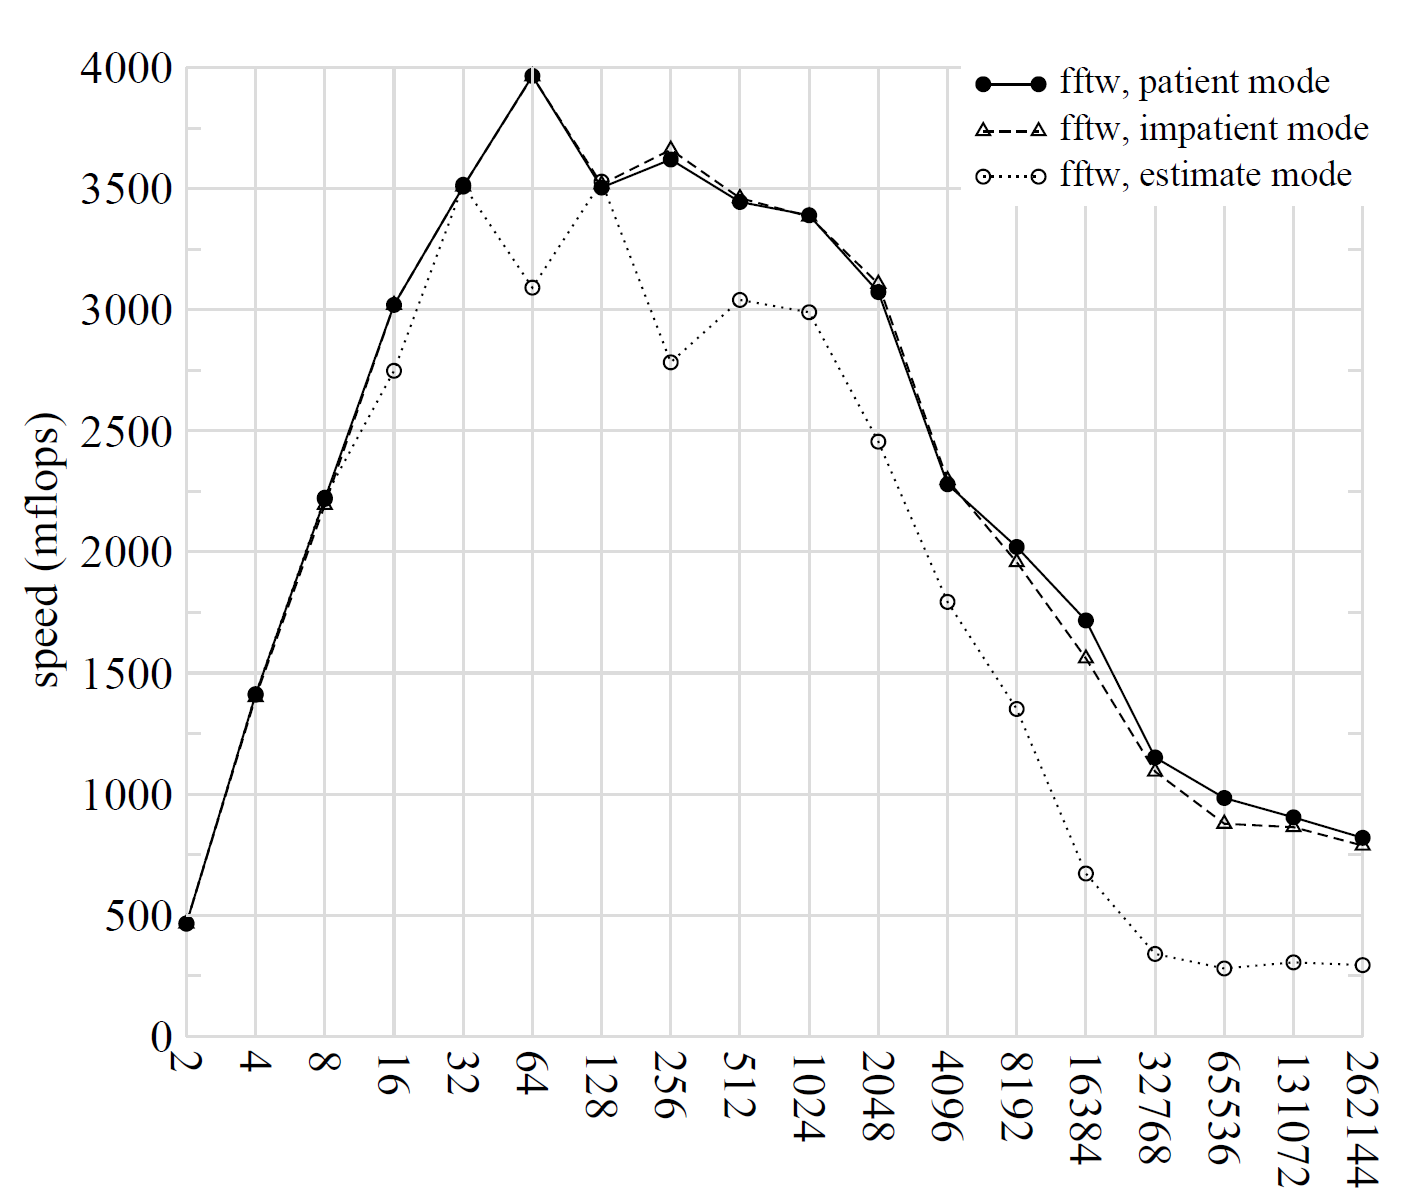
\includegraphics[width=0.7\textwidth]{figures/Plans_Performance.png}
\caption{Effects of planner flags in FFTW on the execution performance for double-precision 1D complex DFTs, power-of-two sizes, on a 2 GHz PowerPC 970 (G5)\cite{FFTW05}.}
\label{Planner flags}
\end{figure}

\subsubsection{Memory Hierachy: Breadth-First versus Depth-First}
A major challenge when implementing the Cooley\textendash Tukey algorithm is that the input $\textbf{x}$ is discontiguous for a contiguous output $\textbf{X}$ or vice versa.
As a consequence discontiguous memory access and data reordering hinders efficient use of hierarchical  memory architectures.
The execution order is therefore a non obvious aspect of an efficient FFT implementation.

One order distinction among others can be made between recursion and iteration.
As shown in Figure \ref{breadth_first} the Cooley\textendash Tukey algorithm can be represented as a tree of smaller and smaller DFTs.
The tree can be traversed either breadth or depth first.
The traditional Cooley\textendash Tukey algorithm as presented in section \ref{Cooley Tukey section} uses the breadth-first approach.
When dividing the initial DFT of length 8, the traditional approach comes up with both representations of length-4 DFTs.
For large inputs this can mean that parts of generated data for the sub-DFT is already out of cache, leading to cache misses and therefore additional time for reloading data.
In contrast the recursive depth-first approach goes directly down until a base case is reached.
Hence, loaded data in the cache are directly used, leading to fewer cache misses.

In this context the choice of radix is also relevant.
A radix-2 algorithm only halves the length of the input vector.
Hence, the way down to a base case incorporates significantly more steps than for an algorithm of higher radix.
Due to the low rate of reducing necessary data for the computation algorithms of small radices can also suffer from cache misses.
FFTW encompasses a breadth-first as well as depth-first approaches. However, it favors the recursive approach. Even though there is no fixed radix-length, 32 is typical \cite{JohnsonFr08:burrus}.

\begin{figure}[h] 
\centering
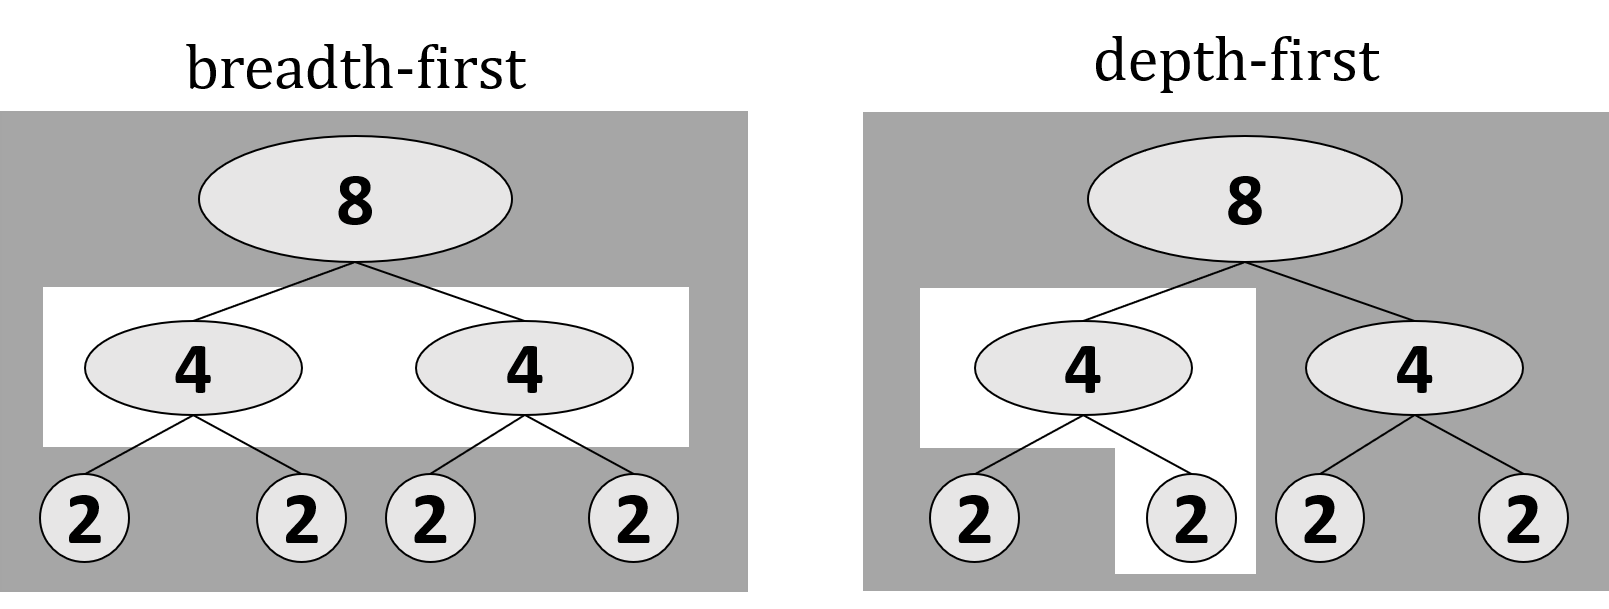
\includegraphics[width=0.7\textwidth]{figures/beadth_first.png}
\caption{Traditional iterative breadth-first versus recursive depth-first orderung for radix-2 FFT of size 8\cite{JohnsonFr08:burrus}. }
\label{breadth_first}
\end{figure}

\subsubsection{Performance and Comparison with Intel MKL}
FFTW is a library for scientific computing, performance is therefore an important aspect.
The authors benchmarked their implementation against most other implementations of the FFT \cite{JuliaCon}.
The results are published on the FFTW homepage \cite{FFTWspeed}.
However, these benchmark date back to 2003 and are not considered here.
The most competitive implementation today is Intel's Math Kernel Library (Intel MKL) \cite{khokhriakov2018novel},\cite{JuliaCon}.

In \cite{khokhriakov2018novel} the authors compare FFTW-2.15, FFTW-3.3.7, and Intel MKL FFT for 2D DFTs of complex power-of-two inputs using 36 threads.
In this setting FFTW-2.1.5 showed better average speed than FFTW-3.3.7.
The authors explain it by a less architecture-specific approach in FFTW-2.1.5 compared to FFTW-3.3.7. Figure \ref{MKL_speed} shows the comparison between FFTW-2.1.5 and Intel MKL FFT3.
Intel's library shows higher peak performance as well as higher average speed.
However, it has significantly higher variation in speed, because the library is optimized to specific DFT-lengths.
FFTW-2.1.5. shows steadier performance and is faster in 162 out of 1000 problem sizes\cite{khokhriakov2018novel}.
For non-power-of-two, FFTW still outperforms Intel MKL according to Steven G. Johnson in a talk at the JuliaCon 2019 \cite{JuliaCon}.

\begin{figure}[h] 
\centering
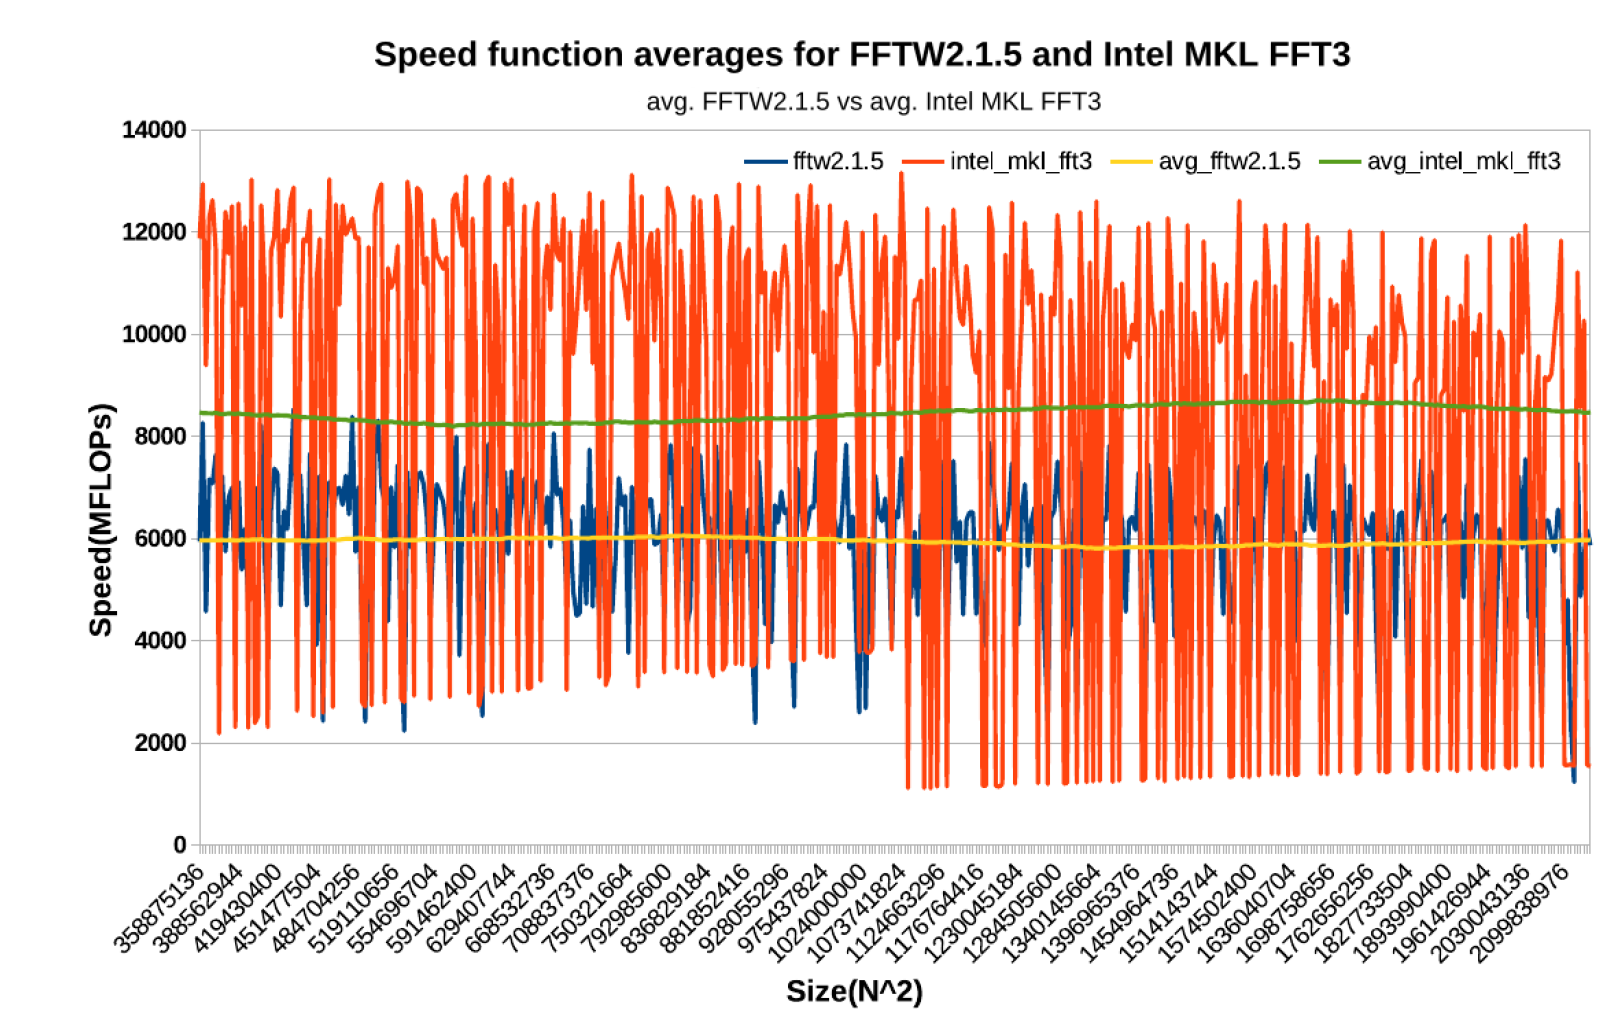
\includegraphics[width=0.7\textwidth]{figures/MKL_speed.png}
\caption{Speed functions of FFTW-2.1.5 and Intel MKL FFT3 and average speeds\cite{khokhriakov2018novel}. }
\label{MKL_speed}
\end{figure}

The results of the performance benchmark are consistent with the initial goals of FFTW, as the authors prioritized generality, which also applies to the length of the DFTs over specific optimization.

\subsection{Limitations and Outlook}
Although the FFT provides detailed information about the frequency contents of a given signal by calculating the DFT, it cannot detect when a certain frequency occurs.
There are many signals of interest that are not stationary in frequency.
A melody played by a single instrument could be (in a simplified way) described as the evolution in time of the frequency characterizing  the note.
The classical FFT cannot provide this information\cite{brunton_kutz_2019}, \cite{57199}. 

In order to gain information of the time resolution of frequency, the DFT is performed on a specific window, which iterates over the time domain.
Hence, a DFT of each window is created, giving frequency information in the specific time frame.
This is a so called short-time Fourier transform (STFT).
Gabor proposed to use Gaussian window functions.
Figure \ref{Gabor_transform} shows how a Gaussian function centered at $\tau$  translated over the time signal to take a DFT in the domain $[\tau -a, \tau +a]$.
The choice of an appropriate window function is essential for the properties of the STFT and the subject of deep mathematical discussions\cite{57199}.  


\begin{figure}[h] 
\centering
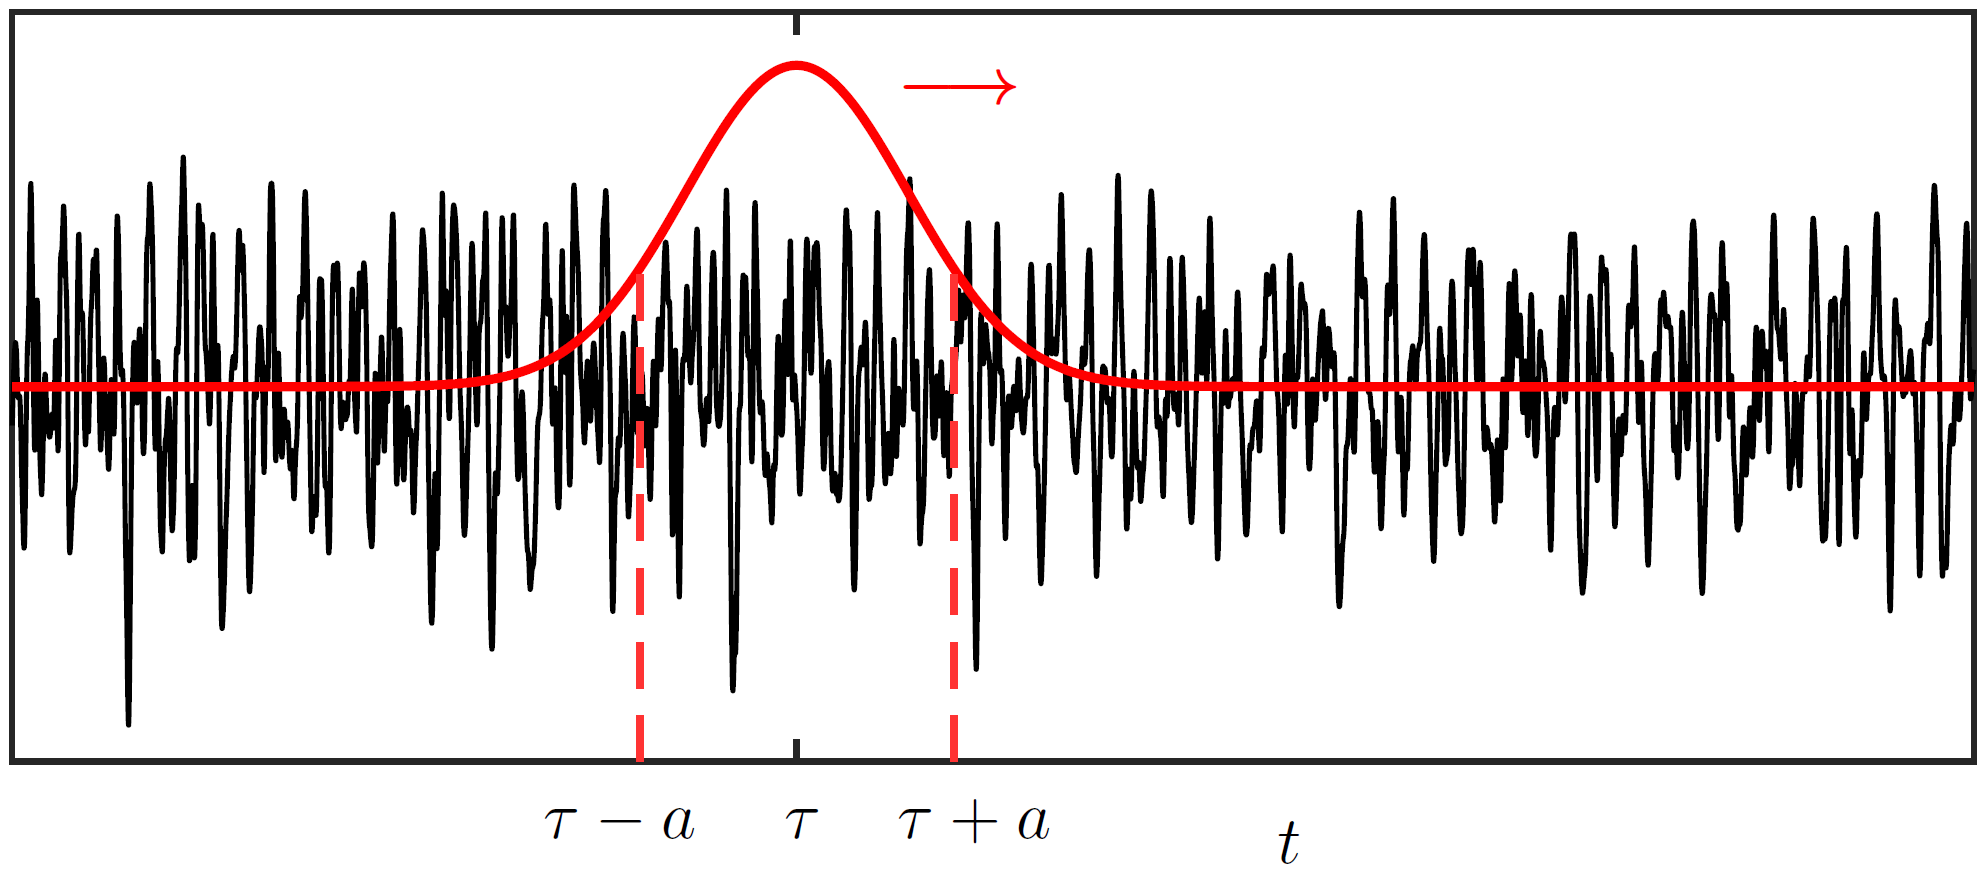
\includegraphics[width=0.7\textwidth]{figures/Gabor.png}
\caption{Illustration of the Gabor transform: A Gaussian window function translates over a time signal to compute the STFT \cite{brunton_kutz_2019}.}
\label{Gabor_transform}
\end{figure}

The visualization of the STFT is the spectrogram.
It is often plotted in 2D and the colors indicate the intensities of the frequencies at a specific time.
An example for an audio signal is given in Figure \ref{Spectrogram}.

\begin{figure}[h] 
\centering
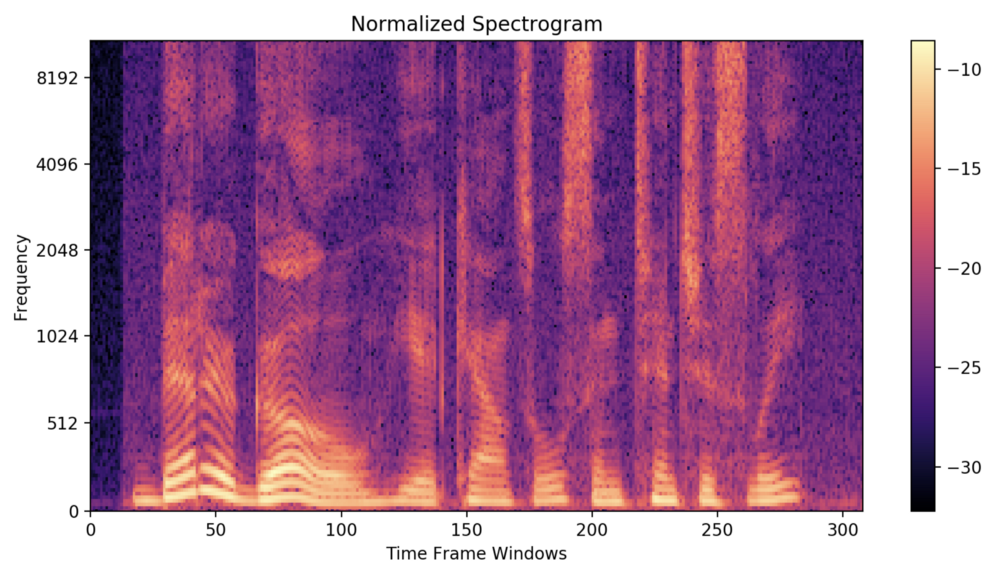
\includegraphics[width=0.7\textwidth]{figures/spectrogram.png}
\caption{Spectrogram of an audio signal where the colors represent certain frequency intensities in time\cite{Spectrogram}. }
\label{Spectrogram}
\end{figure}

The size of the interval $[\tau -a, \tau +a]$ in Figure \ref{Gabor_transform} determines the time resolution of the STFT.
However, the smaller the interval chosen, the lesser information it contains about the frequencies.
This is the fundamental uncertainty principle: It is impossible to attain both high time and frequency resolution.
The Fourier transform is perfectly resolved in frequency without any information about time.
The time series in contrast is perfectly resolved in time without any frequency information.
The spectrogram resolves both but with lower resolution in each domain.
Basically, the product of information in frequency and information in time is bounded by a constant\cite{brunton_kutz_2019}.

The most important approach to get a better trade-off between time and frequency resolution are wavelet transforms.
Wavelets transforms allow multiresolution analysis of signals.
Different time and frequency fidelities can be used for different frequency bands as depicted in Figure \ref{Uncertainty}(d).
Typically higher time resolutions are also used for higher frequencies.
Wavelet transforms are, in particular, useful for multiscale processes, which can be found in epidemiology, seismology, or turbulence.
Wavelets are furthermore the leading approach for image compression\cite{brunton_kutz_2019},\cite{57199}.

\begin{figure}[h!] 
\centering
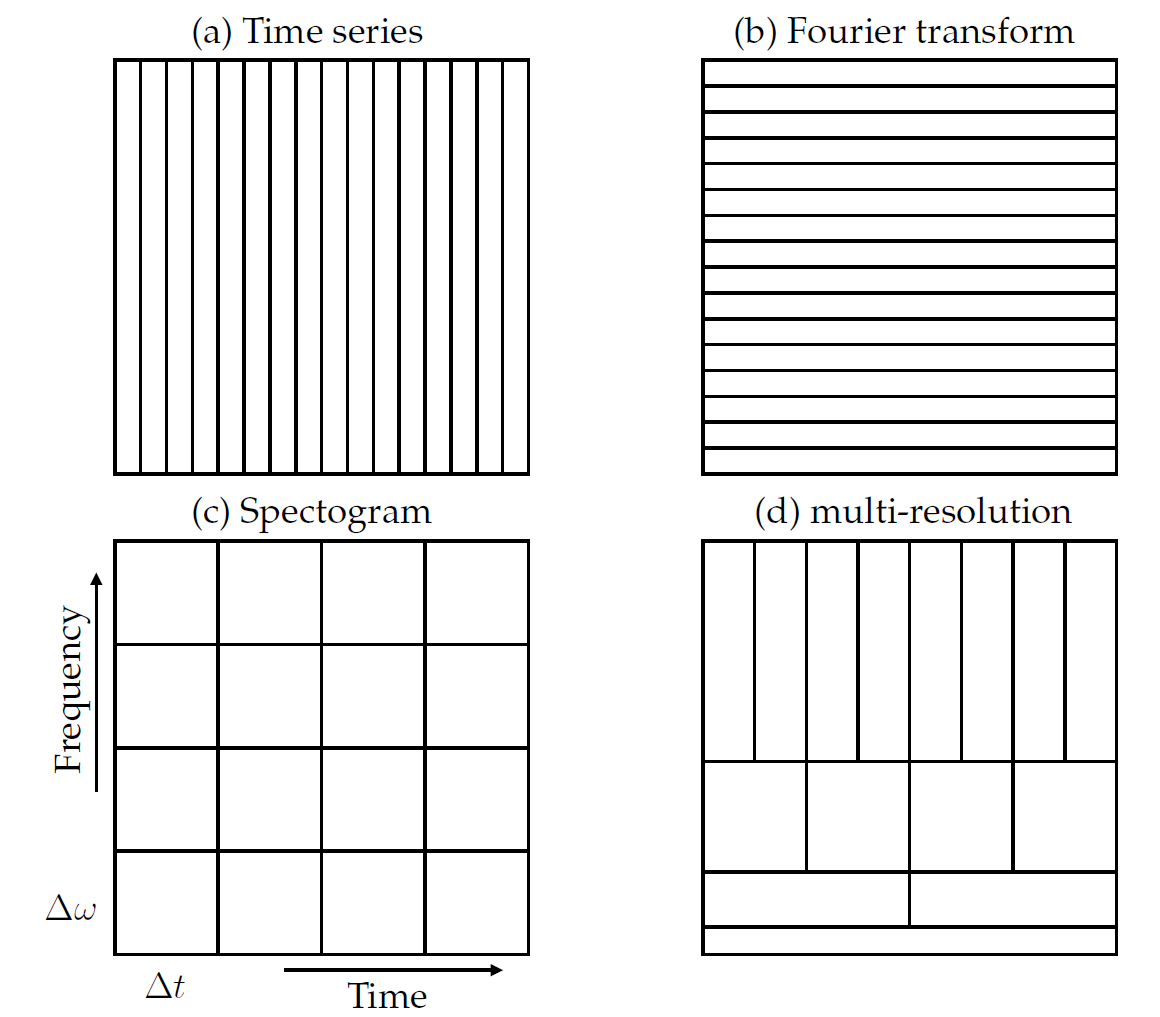
\includegraphics[width=0.7\textwidth]{figures/Uncertainty.png}
\caption{According to the uncertainty principle resolution in time limits resolution in frequency and vice versa.
Multiresolution approaches resolve high frequency bands also high in time\cite{brunton_kutz_2019}.  }
\label{Uncertainty}
\end{figure}

\section{Conclusion}
The FFT is considered to be one of the most important algorithms of the 20th century \cite{FFTTop10},\cite{brunton_kutz_2019}.
Its significance can be grasped, by the vast variety of its applications: signal processing, data analysis, communication, data compression, and many more.

In its core the FFT allows us to compute the DFT very efficiently.
Thus, it enables a fast transition from the time into the frequency domain and vice versa. Necessary computations can be reduced from $\mathcal{O}(N^2)$ to $\mathcal{O}(N \log(N))$. The most important and widely used FFT algorithm is the Cooley\textendash Tukey algorithm.
It splits the initial problem into smaller DFTs, which are reconnected by twiddle factors.
The computational savings in this approach come from intrinsic symmetries in the DFT that allow the reuse of computations.
Important classifications of the Cooley\textendash Tukey algorithm are whether the initial data are split in the time or frequency domain (DIT versus DIF) and in how many sub-DFTs the intial problem is split "radix-X".
Furthermore the problem can be recursively solved depth-first or iteratively breadth-first.

Beside the Cooley\textendash Tukey algorithm, there are other FFT-algorithms of importance.
Many are tailored for special problems.
The fast Hatley transform specializes in real input data and leads to more efficient computations than the Cooley\textendash Tukey algorithm.
Rader's algorithm allows the computation of DFTs of prime size, by using mathematical convolutions.

In addition to a mathematically efficient algorithm, good implementations are needed.
FFTW is one of the leading libraries implementing the FFT.
It is designed to be very flexible in regard to the DFT that is to be solved.
As it used code generation and performance measurements to find an optimal "plan" for each architecture, FFTW is also competitive in terms of performance.

The classical FFT does not give information about the change of frequency in time.
However, splitting the initial time domain and performing separate FFTs leads to the STFT, which allows us to render frequencies dependent on time.
The uncertainty principle limits the amount of information that can be gained from a signal.
Hence better resolution in time leads directly to worse resolution in frequency and vice versa.


\bibliographystyle{plain}
\bibliography{citations}

\end{document}

